\chapter{Programmbeschreibung}\label{ch:programmbeschreibung}

\section{UML-Diagramme}\label{sec:uml}
\begin{figure}[htb]
    \centering
    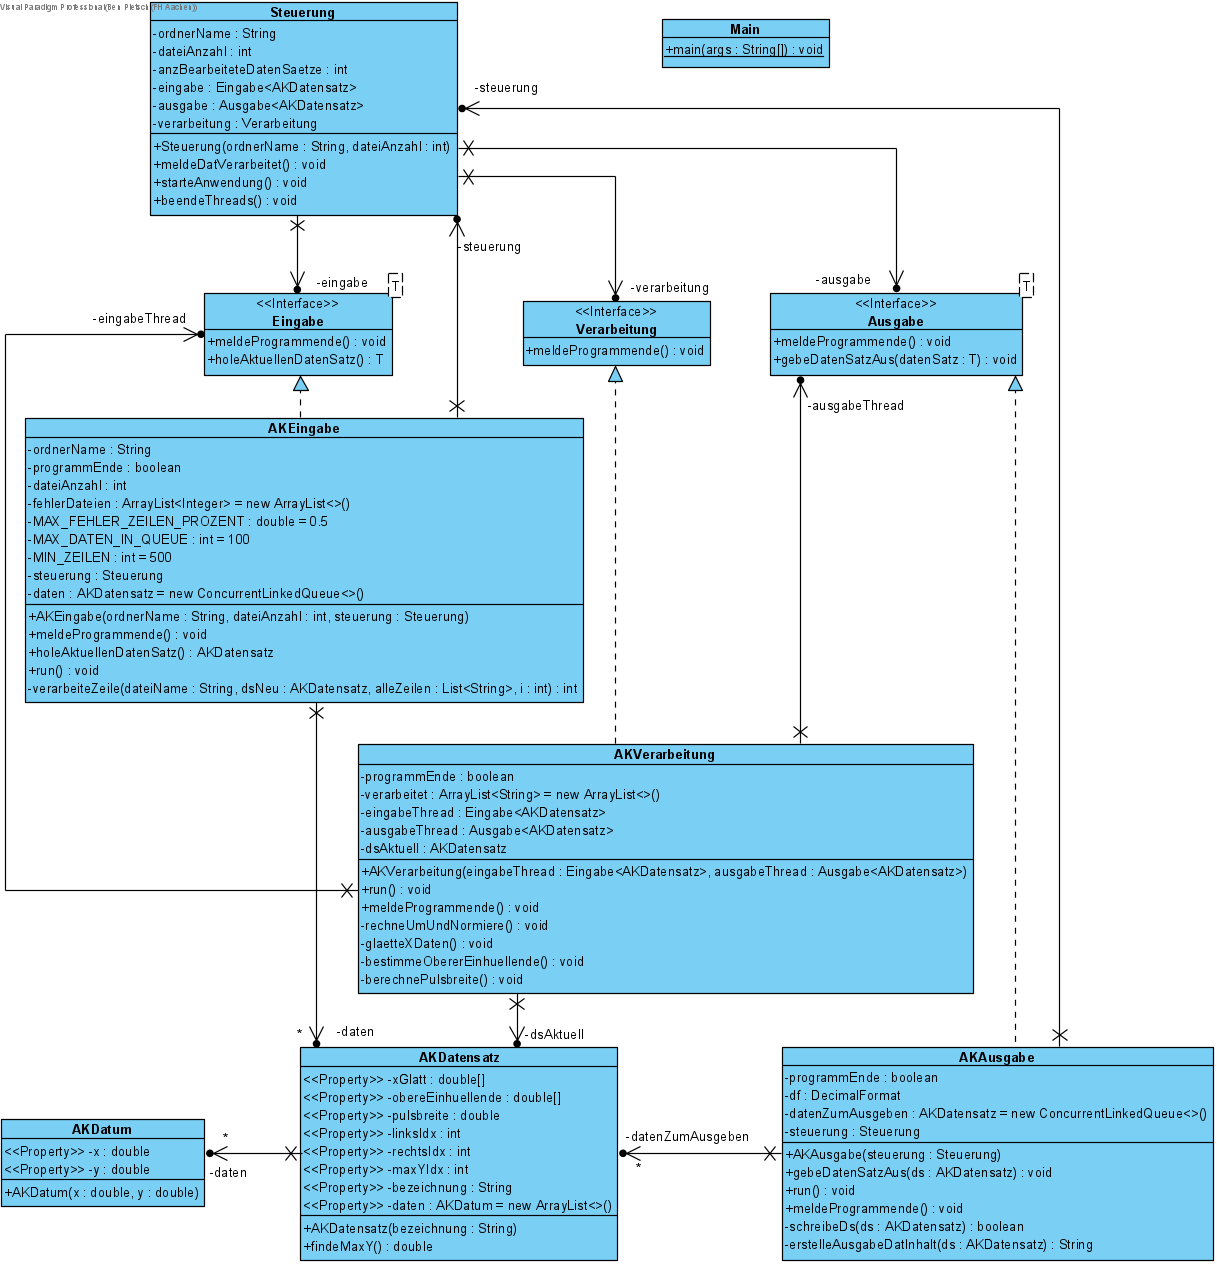
\includegraphics[width=\linewidth]{images/ClassDiagram1}
    \caption{
        Klassendiagramm.
    }
    \label{fig:klassen-dia}
\end{figure}

\section{Struktogramme}\label{sec:strukto}

%\begin{figure}[htb]
%    \centering
%    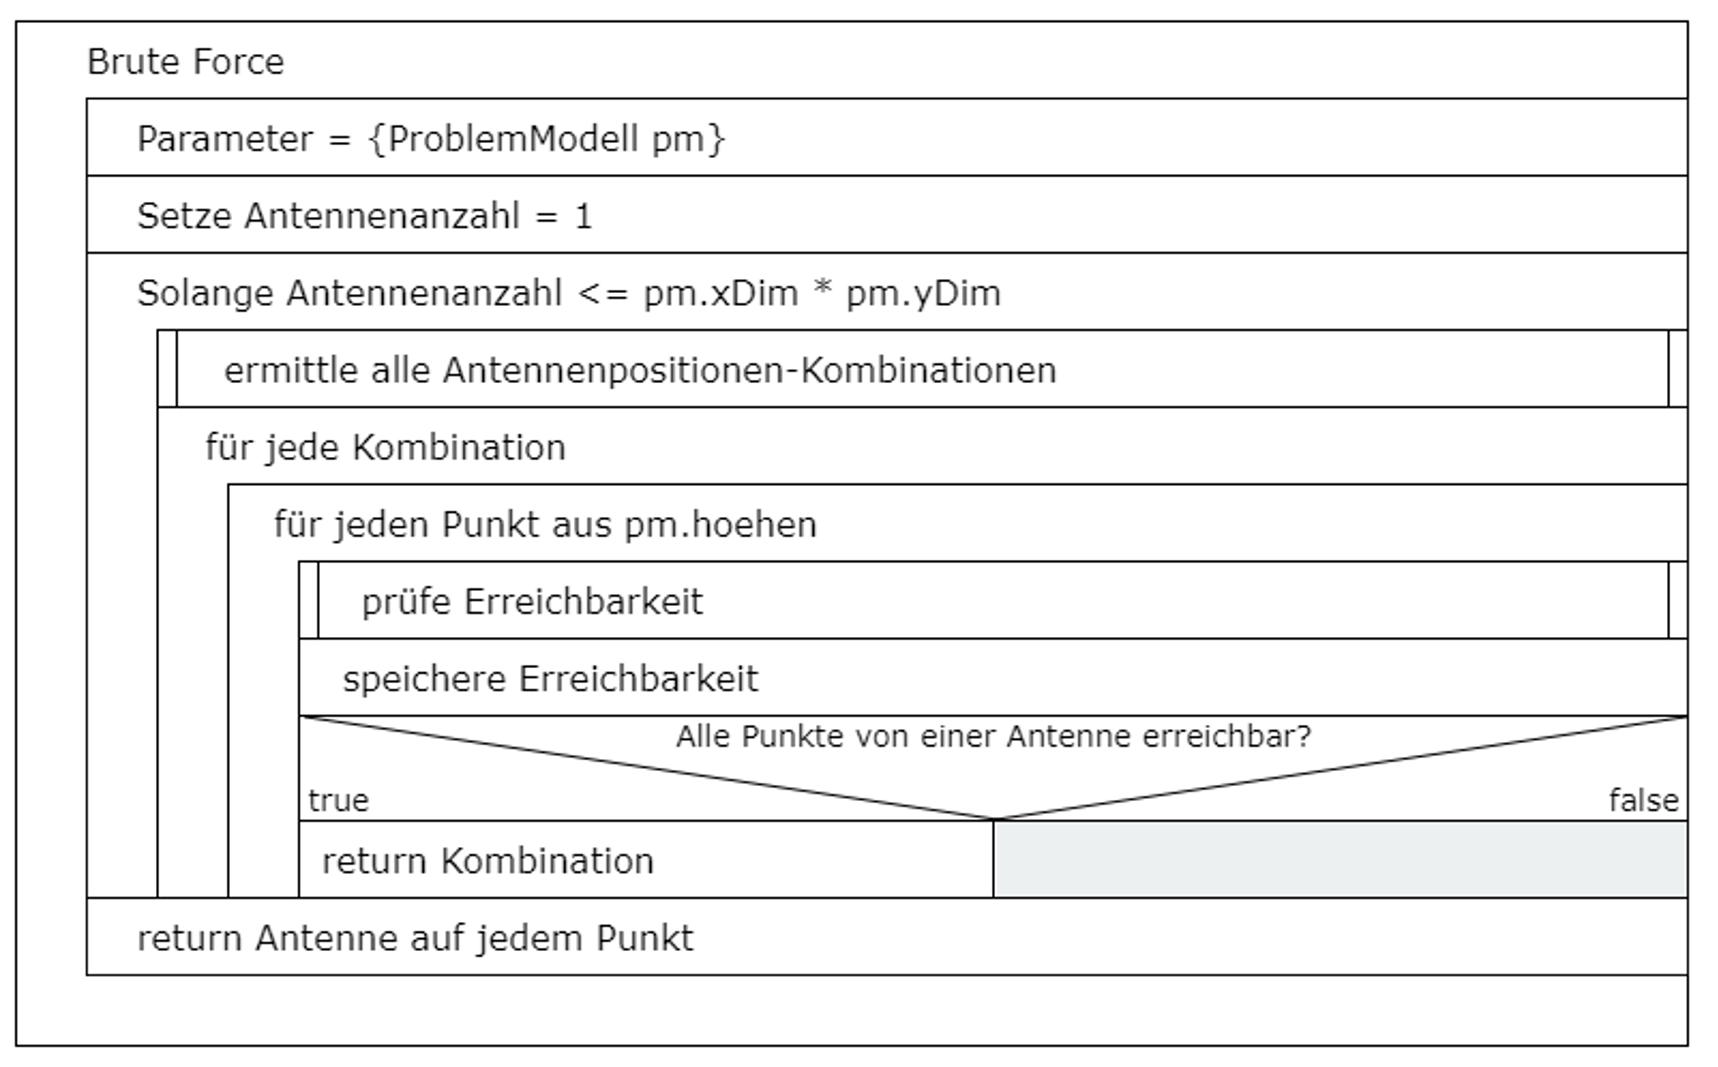
\includegraphics[width=\linewidth]{images/Struktogram}
%    \caption{
%        Generelle Struktur des Lösungs-Algorithmus.
%    }
%    \label{fig:github}
%\end{figure}

\section{Entwicklungsdokumentation}\label{sec:entwicklerdokumentation}
Im Abgabe-Ordner befindet sich ein Verzeichnis mit dem Namen \glqq JavaDoc\grqq{}.
Mit einem Doppelklick auf die darin enthaltene Datei \glqq index.html\grqq{} öffnet sich die Dokumentation im Web-Browser.